\section{Theoretical Analysis}
\label{sec:analysis}
First of all, we performed an operating point analysis in order to check if the transistor was operating in the forward active region.
\begin{table}[h!]
  \centering
  \begin{tabular}{|l|r|}
    \hline    
    {\bf Name} & {\bf Values} \\ \hline
    \input{th_data_tab} 
  \end{tabular}
  \caption{Operating point analysis results.}
  \label{tab:data}
\end{table}

As we can see, VCE is greater than VBEON (0.7V), so we're good to go.
\subsection{Gain Stage}
For the gain stage, the analysis of the incremental circuit yielded the following results:
\begin{table}[h]
  \centering
  \begin{tabular}{|l|r|}
    \hline    
    {\bf Name} & {\bf Values} \\ \hline
    \input{gain_tab} 
  \end{tabular}
  \caption{Gain stage theoretical results}
  \label{tab:gain}
\end{table}

We can clearly see the need for an output stage, given the magnitude of the output impedance. The gain is also significant, and we'll strive for a unitary gain in the output stage in order not to sacrifice this.
\begin{table}[h!]
  \centering
  \begin{tabular}{|l|r|}
    \hline    
    {\bf Name} & {\bf Values} \\ \hline
    \input{outoper_tab} 
  \end{tabular}
  \caption{Operating point analysis results.}
  \label{tab:data2}
\end{table}

\subsection{Output Stage}
\begin{table}[h]
  \centering
  \begin{tabular}{|l|r|}
    \hline    
    {\bf Name} & {\bf Values} \\ \hline
    \input{output_tab} 
  \end{tabular}
  \caption{Output stage theoretical results}
  \label{tab:output}
\end{table}
As desired, the input impedance of this stage is much bigger than the output impedance of the gain stage. This means that the circuit experiences very little signal loss. As well, the output impedance of this stage is desirably low when compared to the 8 Ohm of the speakers.
At last, the total circuit gain results.
\begin{table}[h]
  \centering
  \begin{tabular}{|l|r|}
    \hline    
    {\bf Name} & {\bf Values} \\ \hline
    \input{circuit_tab} 
  \end{tabular}
  \caption{Total circuit theoretical gain results}
  \label{tab:output}
\end{table}

\begin{figure}[!h] \centering
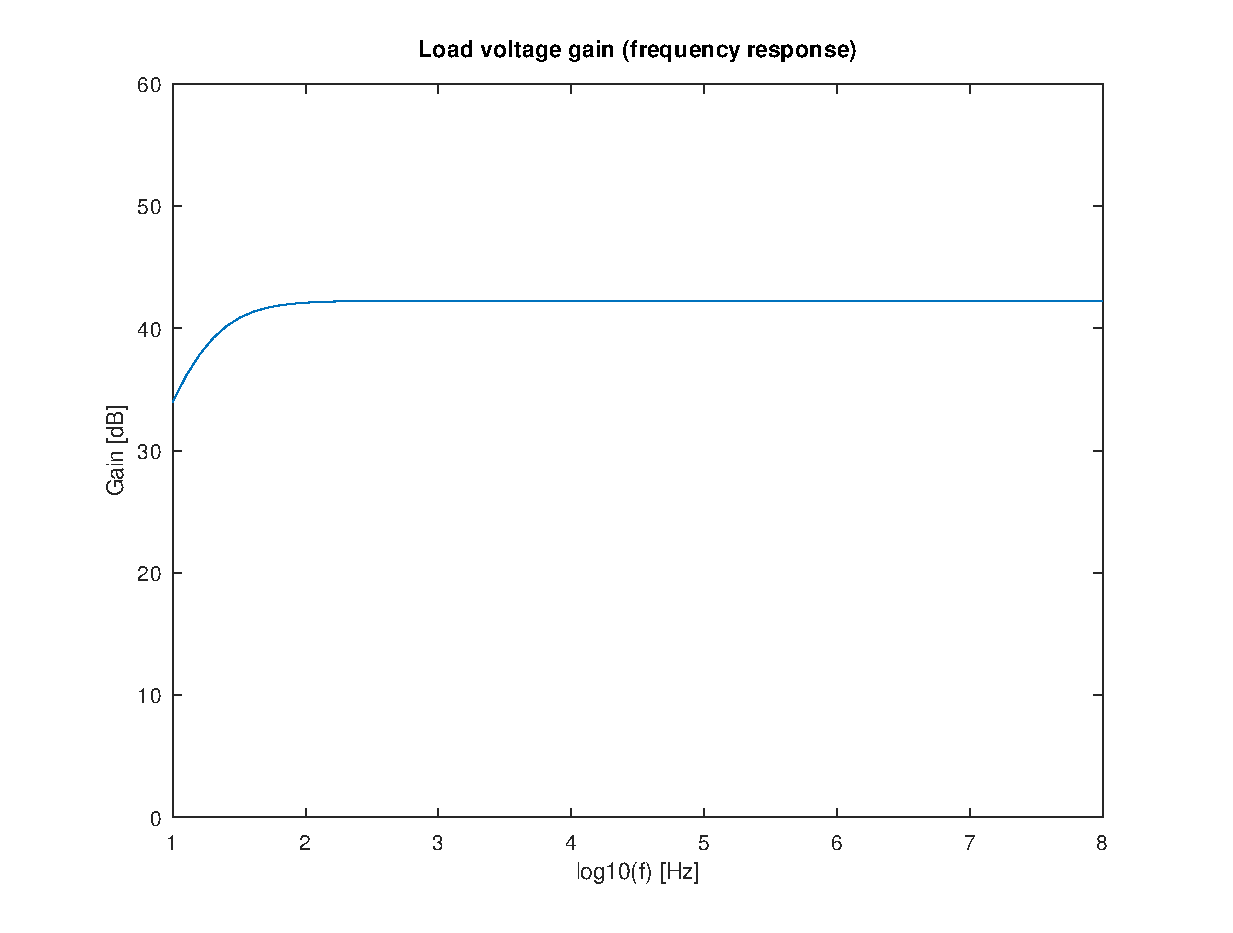
\includegraphics[width=0.6\linewidth]{Gain.eps}
\caption{Load output voltage gain (frequency response).}
\label{fig:gainfreq}
\end{figure}

\begin{figure}[!h] \centering
\includegraphics[width=0.6\linewidth]{Phase.eps}
\caption{Load output voltage phase difference (frequency response).}
\label{fig:phasefreq}
\end{figure}

\begin{table}[h]
  \centering
  \begin{tabular}{|l|r|}
    \hline    
    {\bf Name} & {\bf Values} \\ \hline
    \input{frequency_tab} 
  \end{tabular}
  \caption{Gain for medium frequencies and lower cut-off frequency of the output voltage signal.}
  \label{tab:freq}
\end{table}
